\chapter{面向问题复述识别的模型综合能力鲁棒性研究}\label{5.point3}

上一章采用定向数据增强方法扩充了大量高质量、多元化的训练样本,强化了问题复述识别模型的精细语义感知能力,一定程度上提高了模型的鲁棒性。
鲁棒性能够反映出模型的实用能力,尤其在语法灵活、语义多样的中文领域,对模型鲁棒性的研究尤为重要。
然而,上一章的实验仅得出模型鲁棒性有所提升的简单结论,缺少对其鲁棒性变化的详细分析与探讨。
为此,本章构造了一个符合中文语言学特征的评估数据集CQM$_{robust}$,用以系统化评估问题复述识别模型的能力及鲁棒性。
CQM$_{robust}$包含3种语言特征、13个测试子类,共计32个测试项,且其所有数据均来源于搜索引擎中的真实提问。
大量的实验表明,CQM$_{robust}$比传统数据集难度更大,更具有挑战性,
且能够按不同语言现象对模型进行详细评估,有助于诊断现有模型的优势和劣势。
下面将详细介绍本章的研究动机、数据构造方案以及实验分析。

\section{引言}

在过去的几年里,预训练语言模型在NLP领域引起了轰动,其在许多传统的数据集上取得了优异的性能,
包括问题复述数据集Quora\cite{iyer2017first}、LCQMC\cite{liu2018lcqmc}、BQ\cite{chen2018bq}和AFQMC\footnote{蚂蚁技术探索会议(ATEC)开发者竞赛}。
然而,与其性能表现不一致的是,目前最先进的模型在现实世界的场景中仍会出现令人惊讶的错误。
如表~\ref{table5-1}~所示( {\kai\colorbox{lightgreen}{\color{darkgreen}绿色}} 和 {\kai\colorbox{lightred}{\color{darkred}红色}} 部分标记出问题之间的细微差别),
第一个例子中,RoBERTa模型无法区分两个问题中{\kai“蔬菜”}和{\kai“绿色蔬菜”}之间的细微差异,从而将这两个问题误判为语义等价的复述关系;
第三个例子中,模型没有判断出{\kai“监狱”}与{\kai“牢房”}两个词为同义,从而将其误判为非复述关系。
由此可见,现有模型不能以灵活方式处理简单的案例。

% 表: 例子
\begin{table}
    \caption{CQM$_{robust}$数据样例}
    % \begin{spacing}{1.1}
    % \small
    \centering
    \newcommand{\tabincell}[2]{\begin{tabular}{@{}#1@{}}#2\end{tabular}}
    \begin{tabular}{llcc}
    \toprule[0.7pt]
     \textbf{问题1} & \textbf{问题2} & \textbf{标签} & \textbf{RoBERTa} \\
    \midrule[0.7pt]
    婴儿吃什么蔬菜好? & 婴儿吃什么\colorbox{lightgreen}{\color{darkgreen}绿色}蔬菜好?\;\  & 0 & 1 \\\hline
    心率过\colorbox{lightred}{\color{darkred}慢}有什么危害 & 心率过\colorbox{lightgreen}{\color{darkgreen}快}有什么危害 & 0 & 1 \\\hline
    求关于\colorbox{lightred}{\color{darkred}监狱}的电视剧\quad\ & 求关于\colorbox{lightgreen}{\color{darkgreen}牢房}的电视剧 & 1 & 0 \\
    
        
    \bottomrule[0.7pt]
    
    \end{tabular}
    \label{table5-1}
    % \end{spacing}
\end{table}

近期,关于神经网络模型鲁棒能力的研究吸引了大量学者的关注。
早期的研究工作通过创建某种类型的对抗性样本,并以此评估神经模型的鲁棒性\cite{jia2017adversarial,alzantot2018generating,ren2019generating,jin2020bert}。
如表~\ref{table5-1}~中的样例,对抗性样本指的是在原始样本中加入一些不影响人类识别但却容易愚弄模型的扰动。
也有一些研究通过人机对抗的方式构造对抗性样本,
如Nie等利用人类与模型在多轮循环对抗中构建的对抗性自然语言推理数据集(Natural Language Inference,简称NLI)\cite{nie2019adversarial},
其在多轮对抗中数据集难度逐渐上升,对NLI模型的能力提出新的挑战。
此外,相关研究开始尝试借助对抗训练的方案\cite{min2020syntactic,bao2021defending,wang2021natural}抵御对抗性样本的攻击。
这些努力更加有利于发现和解决模型鲁棒性缺陷。

然而,以往关于模型鲁棒性的研究仅针对某中特定场景下的数据,或是只使用了少量的数据变化方法,缺乏综合性的评估方案。
合理的评估方案应当以多样化的数据综合评估模型的表现,而不是单一的攻击模型某种能力漏洞。
为了更全面地评估模型的性能,Ribeiro等提出了一种用于NLP模型行为测试的方法和配套工具CHECKLIST\cite{ribeiro2020beyond}。
用户可以借助其定制测试列表,从多个抽象概念中生成测试样本。
复旦大学发布的模型鲁棒性评测平台TextFlint\cite{gui2021textflint}也为模型鲁棒性评测提供了一站式解决方案。
然而,CHECKLIST和TextFlint以模板化方式大量生产的样本不能客观地代表真实世界的自然语言,
且缺乏针对特定语言和特定任务的语法现象分析。

为此,本章创建了一个开放领域的中文数据集CQM$_{robust}$,用于评估问题复述识别模型的综合能力及鲁棒性。
如表~\ref{table5-2}~所示,CQM$_{robust}$包含3大类语言特征、13个测试子类,共计32个测试项。
并且CQM$_{robust}$中的所有问题均源于百度商业搜索引擎\footnote{http://www.baidu.com/}中的用户真实提问,
而非刻意通过人工撰写的非自然问句,
这有利于客观评价模型的实际应用能力。
本章的主要贡献有:

\begin{enumerate}
    \item 
    构建了一个系统化的中文问题复述识别评估基准CQM$_{robust}$,其中所有问题均为百度搜索引擎真实数据。
    \item 
    CQM$_{robust}$比传统数据集更加具有挑战性,并且能够按语言现象诊断模型,区分不同模型的优势和劣势。
\end{enumerate}

本章的组织形式如下:第1节为引言部分;第2节详细介绍CQM$_{robust}$数据集的结构体系;第3节介绍了数据集的构造方案;第4节介绍实验部分并进行结果分析;第5节对本章内容进行总结。


\section{CQM$_{robust}$体系结构}

CQM$_{robust}$旨在按照中文语言现象对模型进行详细评估,这些语言现象对评价模型的能力至关重要。
因此,本章将测试数据归纳为3种符合语言学特征的类别,包括词法特征(Lexical Features)、
句法特征(Syntactic Features)和语境特征(Pragmatic Features)。
如表~\ref{table5-2}~所示,本节将介绍CQM$_{robust}$各个能力类别的详细特点。

\subsection{词法特征}\label{5.2.1 词法特征}

词法特征考察模型对各类词汇理解程度。
词是独立但有意义的最小语义单元,一个词的变化也会改变整个句子的意义。
本章将词法特征归纳为如下6个子类别:

% 表: CQM\textsubscript{robust}数据集统计
\begin{table}[!h]
    \caption{CQM\textsubscript{robust}评估体系及基线模型评估结果}
    % \tiny
    \centering
    \newcommand{\tabincell}[2]{\begin{tabular}{@{}#1@{}}#2\end{tabular}}
    \resizebox{155mm}{108mm}
    {
    \small
    %\begin{adjustbox}{max width=\textwidth}
    \begin{tabular}{c|c|c|c|cccccc|l}
    \toprule[0.7pt]
    %  \textbf{ \tabincell{c}{Coarse-grained\\ Categories}} & \textbf{\tabincell{c}{Fine-grained\\ Categories}} & \textbf{\tabincell{c}{Perturbation\\ Operations}} & \textbf{Examples and Translation} & \textbf{Label} & \textbf{\#Y / \#N} \\
      \textbf{ \tabincell{c}{类别}} & \textbf{\tabincell{c}{子类}} & \textbf{\tabincell{c}{扰动\\操作}} & {\tabincell{c}{\textbf{标签} \\ \#1 / \#0}} &{ \tabincell{c}{BERT\\base}}&{ \tabincell{c}{ERNIE\\base}} & { \tabincell{c}{RoBERTa\\base}}&{ \tabincell{c}{MacBERT\\base}}&{ \tabincell{c}{RoBERTa\\large}}&{ \tabincell{c}{MacBERT\\large}}& \tabincell{c}{样例及翻译} \\
    \midrule[0.7pt]
    
    % Lexical
    
    % basic
    \multirow{55}*{{\rotatebox{90}{\textbf{词法}}}} & \multirow{22}*{\tabincell{c}{基础\\词汇}} & 插入名词 &
     -/539
    &
    41.4±3.4 & 40.8±2.1 & \underline{43.0±0.7} & 41.4±2.5 & \textbf{45.4±4.1} & 37.3±2.4 &
     \tabincell{l}{\textbf{E1}: \label{example:E1}鸡蛋怎么炒好吃\;/\; 鸡蛋\colorbox{lightgreen}{\color{darkgreen}面}怎么炒好吃 \\
    \quad\;\;\, how to fry eggs\;/\; how to fry egg 
     \colorbox{lightgreen}{\color{darkgreen}noodles}}
     \\\cline{3-11}
    
     & & 插入动词& 
     -/131
     &
     \underline{39.4±0.4} & 33.8±2.6 & 37.4±2.0 & 35.9±2.7 & \textbf{39.9±3.1} & 29.5±3.8 &
     \tabincell{l}{\specialrule{0em}{0em}{1mm}\textbf{E2}: \label{example:E2}伤口用什么好\;/\; 伤口用什么\colorbox{lightgreen}{\color{darkgreen}消毒}好\\
    \quad\;\;\,what is good for the wound\;/\; how to \colorbox{lightgreen}{\color{darkgreen}disinfect} the wound
    }
    \\\cline{3-11}
    
     & & 插入形容词 & 
     -/458
     &
     23.5±1.9 & 19.2±3.7 & \textbf{26.9±4.4} & \underline{23.9±4.2} & 18.1±2.4 & 10.4±2.1 &
     \tabincell{l}{\specialrule{0em}{0em}{1mm}\textbf{E3}: \label{example:E3}有哪些类型的app\;/\; 有哪些类型的\colorbox{lightgreen}{\color{darkgreen}移动}app\\
     \quad\;\;\,what are types of apps\;/\; what are types of \colorbox{lightgreen}{\color{darkgreen}mobile} apps
    }
    \\\cline{3-11}
    
     & & 插入副词& 
      -/302
     &
     3.7±0.5 & 4.2±0.5 & 3.8±0.6 & \underline{4.4±1.2} & \textbf{5.8±1.5} & 3.1±1.1 &
     \tabincell{l}{\specialrule{0em}{0em}{1mm}\textbf{E4}: \label{example:E4}为什么打嗝\;/\; 为什么\colorbox{lightgreen}{\color{darkgreen}老}打嗝\\
     \quad\;\;\,why burp\;/\; why \colorbox{lightgreen}{\color{darkgreen}always} burp
    }
    \\\cline{3-11}
    
    %/v./adj./adv. 
     & & 替换名词 & 
      -/702
     &
     86.6±0.3 & 86.7±0.1 & 88.3±0.3 & \underline{88.8±1.2} & \textbf{89.4±1.6} &  87.8±0.7&
     \tabincell{l}{\specialrule{0em}{0em}{1mm}\textbf{E5}: \label{example:E5}申请美国\colorbox{lightred}{\color{darkred}绿卡}流程\;/\; 申请美国\colorbox{lightgreen}{\color{darkgreen}签证}流程\\
    \quad\;\;\,U.S. \colorbox{lightred}{\color{darkred}green card} application process\;/\; U.S.  \colorbox{lightgreen}{\color{darkgreen}visa} application process
    }
    \\\cline{3-11}
    
     & & 替换动词& 
      -/466
     &
     71.7±1.1 &77.6±0.8 & 76.9±0.4 & 76.5±1.2 & \underline{81.0±1.6} & \textbf{81.5±2.2} &
     \tabincell{l}{\specialrule{0em}{0em}{1mm}\textbf{E6}: \label{example:E6}为什么\colorbox{lightred}{\color{darkred}下蹲}膝盖疼\;/\; 为什么\colorbox{lightgreen}{\color{darkgreen}下跪}膝盖疼\\
     \quad\;\;\,why knee pain when \colorbox{lightred}{\color{darkred}squatting}\;/\; why knee pain when \colorbox{lightgreen}{\color{darkgreen}kneeling}
    }
    \\\cline{3-11}
    
     & & 替换形容词 & 
      -/472
     &
     74.3±2.1 & 80.0±1.0 & 77.6±0.7 & 81.6±0.5 & \textbf{82.7±1.1} & \underline{82.7±1.6} &
     \tabincell{l}{\specialrule{0em}{0em}{1mm}\textbf{E7}: \label{example:E7}耳朵出血\colorbox{lightred}{\color{darkred}严重}吗\;/\; 耳朵出血\colorbox{lightgreen}{\color{darkgreen}正常}吗\\
     \quad\;\;\,is the ear bleeding \colorbox{lightred}{\color{darkred}serious}\;/\; is the ear bleeding \colorbox{lightgreen}{\color{darkgreen}normal}
    }
    \\\cline{3-11}
    
    & & 替换副词& 
     -/188
    &
    19.1±6.1 & 19.3±4.4 & 16.3±3.8 & 23.9±4.6 & \textbf{59.0±4.0} & \underline{56.2±2.0} &
     \tabincell{l}{\specialrule{0em}{0em}{1mm}\textbf{E8}: \label{example:E8}为什么会\colorbox{lightred}{\color{darkred}经常}头晕\;/\; 为什么会\colorbox{lightgreen}{\color{darkgreen}有点}头晕\\
     \quad\;\;\,why \colorbox{lightred}{\color{darkred}regularly} feel dizzy\;/\; why  \colorbox{lightgreen}{\color{darkgreen}slightly} feel dizzy
    }
    \\\cline{3-11}
    
     & & 替换数词&  
      -/1116
     &
     83.2±1.4 & \underline{91.4±0.4} & 85.9±1.8 & 87.2±0.9 & 88.1±0.5 & \textbf{91.9±1.1} &
     \tabincell{l}{\specialrule{0em}{0em}{1mm}\textbf{E9}: \label{example:E9}血压\colorbox{lightred}{\color{darkred}130}/100高吗\;/\;
     血压\colorbox{lightgreen}{\color{darkgreen}120}/100高吗\\
     \quad\;\;\,is blood pressure \colorbox{lightred}{\color{darkred}130}/100 high \;/\; is blood pressure \colorbox{lightgreen}{\color{darkgreen}120}/100 high}
    \\\cline{3-11}
    
     & & 替换量词&  
      -/22
     &
     {30.3±6.9} & 25.7±5.2 & 33.3±2.6 & \textbf{34.9±2.6} & 27.3±0.0 & \underline{34.8±10.5} &
     \tabincell{l}{\specialrule{0em}{0em}{1mm}\textbf{E10}: \label{example:E10}一\colorbox{lightred}{\color{darkred}束}花多少钱\;/\;
     一\colorbox{lightgreen}{\color{darkgreen}枝}花多少钱\\
     \qquad\, how much is \colorbox{lightred}{\color{darkred}a bunch of} flower \;/\; how much is  \colorbox{lightgreen}{\color{darkgreen}a}flower}
    \\\cline{3-11}
    
     & & 替换词组 &   
      -/197
     &
     \underline{98.0±0.0} & \textbf{98.1±0.2} & 96.6±0.3 & 97.8±0.5 & 97.8±0.2 & 97.5±0 &
     \tabincell{l}{\specialrule{0em}{0em}{1mm}\textbf{E11}: \label{example:E11}如何\colorbox{lightred}{\color{darkred}提高自己的记忆力}\;/\; 如何\colorbox{lightgreen}{\color{darkgreen}增加自己的实力}\\
     \qquad\, how to \colorbox{lightred}{\color{darkred}improve my memory}\;/\; how to \colorbox{lightgreen}{\color{darkgreen}increase my strength}
     }
    
    \\\cline{2-11}
    
    % ner
     & \multirow{8}*{\tabincell{c}{命名\\实体}} & 替换地点 & 
      -/458
     &
     \textbf{96.0±0.6} & \underline{95.7±0.2} & 95.4±0.4 & 95.0±0.4 & 94.7±0.4&94.5±0.5 &
     \tabincell{l}{\specialrule{0em}{0em}{1mm}\textbf{E12}: \label{example:E12}\colorbox{lightred}{\color{darkred}山西}春节习俗 \;/\;\colorbox{lightgreen}{\color{darkgreen}陕西}春节习俗 \\
     \qquad\, \colorbox{lightred}{\color{darkred}Shanxi} spring festival customs\;/\; \colorbox{lightgreen}{\color{darkgreen}Shannxi} spring festival customs}
    \\\cline{3-11}
    
     &  & 替换机构 &  
      -/264
     &
     \textbf{94.9±0.2} & \underline{94.3±0.6} & 91.2±1.4 & 93.4±0.7 & 93.5±0.3 & 93.8±0.1 &
      \tabincell{l}{\specialrule{0em}{0em}{1mm}
      \textbf{E13}: \label{example:E13}\colorbox{lightred}{\color{darkred}北京邮电大学}附近酒店 \;/\; \colorbox{lightgreen}{\color{darkgreen}南京邮电大学}附近酒店\\
     \qquad\, hotels near \colorbox{lightred}{\color{darkred}BUPT}\;/\; hotels near \colorbox{lightgreen}{\color{darkgreen}NJUPT}}
    \\\cline{3-11}
     
     &  & 替换人物 &  
      -/468
     &
     90.3±1.3 & 91.0±0.9  & 88.7±1.6 & 91.4±1.6 & \underline{92.3±1.3}& \textbf{93.2±1.1} &
      \tabincell{l}{\specialrule{0em}{0em}{1mm}
      \textbf{E14}: \label{example:E14}\colorbox{lightred}{\color{darkred}陈龙}的妻子 \;/\; \colorbox{lightgreen}{\color{darkgreen}成龙}的妻子\\
     \qquad\, wife of \colorbox{lightred}{\color{darkred}Long Chen}\;/\; wife of \colorbox{lightgreen}{\color{darkgreen}Jackie Chan}}
    \\\cline{3-11}
     
     &  & 替换物品 &  
      -/170
     &
     83.7±2.6 &\underline{88.2±2.1} & 82.4±6.9 & 83.3±0.3 & 86.0±1.7 & \textbf{88.8±4.4} &
      \tabincell{l}{\specialrule{0em}{0em}{1mm}
      \textbf{E15}: \label{example:E15}\colorbox{lightred}{\color{darkred}iphone 6}多少钱 \;/\; \colorbox{lightgreen}{\color{darkgreen}iphone6x}多少钱\\
     \qquad\, how much is \colorbox{lightred}{\color{darkred}iphone 6}\;/\; how much is \colorbox{lightgreen}{\color{darkgreen}iphone6x}}
    \\\cline{2-11}
     
    % synonym
     & \multirow{8}*{同义词} & 替换名词 &  
      405/-
     &
     51.1±1.1 & 59.7±1.3 & 59.7±2.2 & 60.7±2.0 & \underline{63.3±3.1} &\textbf{71.6±4.0} & 
     \tabincell{l}{\specialrule{0em}{0em}{1mm}
     \textbf{E16}: \label{example:E16}\colorbox{lightred}{\color{darkred}猕猴桃}的功效 \;/\;
      \colorbox{lightgreen}{\color{darkgreen}奇异果}的功效\\
    \qquad\, health benefits of \colorbox{lightred}{\color{darkred}Chinese gooseberry}\;/\;
    health benefits of \colorbox{lightgreen}{\color{darkgreen}Kiwi}}
    \\\cline{3-11}
    
     &  & 替换动词 &  
      372/-
     &
     80.0±0.9& 81.1±1.6 & 82.5±0.0 & 83.2±1.2 & \underline{84.0±2.0} & \textbf{88.1±1.4} &
      \tabincell{l}{\specialrule{0em}{0em}{1mm}
      \textbf{E17}: \label{example:E17}什么果汁可以\colorbox{lightred}{\color{darkred}减肥} \;/\; 什么果汁可以\colorbox{lightgreen}{\color{darkgreen}减重}\\
     \qquad\, what juice can \colorbox{lightred}{\color{darkred}lose weight}\;/\; what juice can \colorbox{lightgreen}{\color{darkgreen}slim}}
    \\\cline{3-11}
     
     &  & 替换形容词 &  
      453/-
     &
     75.7±1.3 & 77.3±1.1 & 78.8±2.5 & 74.8±0.5 & \underline{79.4±3.4} & \textbf{88.5±1.3} &
      \tabincell{l}{\specialrule{0em}{0em}{1mm}
      \textbf{E18}: \label{example:E18}\colorbox{lightred}{\color{darkred}有趣}搞笑的广告词 \;/\; \colorbox{lightgreen}{\color{darkgreen}幽默}搞笑的广告词\\
     \qquad\, \colorbox{lightred}{\color{darkred}funny} advertising words\;/\; \colorbox{lightgreen}{\color{darkgreen}humerous} advertising words}
    \\\cline{3-11}
     
     &  & 替换副词 &  
      26/-
     &
     \underline{98.7±2.1} & \textbf{100.0±0.0} & \textbf{100.0±0.0} & \textbf{100.0±0.0} &\textbf{100±0.0} &\textbf{100.0±0.0} & 
      \tabincell{l}{\specialrule{0em}{0em}{1mm}
      \textbf{E19}: \label{example:E19}\colorbox{lightred}{\color{darkred}总是}想睡觉是为什么 \;/\; \colorbox{lightgreen}{\color{darkgreen}老是}想睡觉是为什么\\
     \qquad\, why \colorbox{lightred}{\color{darkred}always} want to sleep \;/\; why \colorbox{lightgreen}{\color{darkgreen}repeatedly} want to sleep}
    \\\cline{2-11}
    
    % Antonym
     & 反义词 & 替换形容词 & 
      -/305
     &
     50.6±3.4 &69.6±2.9 & 65.0±1.5 & 73.1±4.3 &\textbf{91.7±2.3} &\underline{90.7±2.3} & 
      \tabincell{l}{\specialrule{0em}{0em}{1mm}
      \textbf{E20}: \label{example:E20}什么水果脂肪\colorbox{lightred}{\color{darkred}低} \;/\; 
      什么水果脂肪\colorbox{lightgreen}{\color{darkgreen}高}\\
      \qquad\, what fruit is  \colorbox{lightred}{\color{darkred}low} in fat\;/\;
      what fruit is \colorbox{lightgreen}{\color{darkgreen}high} in fat
      }
      
    \\\cline{2-11}
    % negation
    
     & \multirow{6}*{否定} & 否定动词 &  
      -/153
     &
     69.9±9.6 & 88.9±1.3 & 84.8±2.9 & \textbf{93.3±1.3} & 88.4±0.9 & \underline{91.4±3.4} & 
     \tabincell{l}{\specialrule{0em}{0em}{1mm}
     \textbf{E21}: \label{example:E21}为什么宝宝哭\;/\; 为什么宝宝\colorbox{lightgreen}{\color{darkgreen}不}哭 \\
     \qquad\, why baby cries\;/\; why baby \colorbox{lightgreen}{\color{darkgreen}doesn't} cry
     }
    \\\cline{3-11}
     &  & 否定形容词 &  
      -/139
     &
     73.1±8.5 & 84.2±1.2 & 82.7±1.4 & \underline{88.0±1.5} & 88.0±2.9 & \textbf{89.4±1.0} & 
      \tabincell{l}{\specialrule{0em}{0em}{1mm}
    \textbf{E22}: \label{example:E22}为什么苹果是红的\;/\; 为什么苹果\colorbox{lightgreen}{\color{darkgreen}不是}红的 \\
     \qquad\, why apple is red\;/\; why apple is \colorbox{lightgreen}{\color{darkgreen}not} red }
    \\\cline{3-11}
     
     &  & 否定反义词 & 
      59/-
     &
     29.9±2.5 & 34.4±2.5 & 39.0±1.7 & 31.1±2.5 & \underline{40.7±1.7} & \textbf{53.6±0.9} & 
     \tabincell{l}{\specialrule{0em}{0em}{1mm}
     \textbf{E23}: \label{example:E23}\colorbox{lightred}{\color{darkred}激动}怎么办\;/\; \colorbox{lightgreen}{\color{darkgreen}无法}\colorbox{lightgreen}{\color{darkgreen}平静}怎么办 \\
    \qquad\, what to do if too \colorbox{lightred}{\color{darkred}excited}\;/\; what to do if \colorbox{lightgreen}{\color{darkgreen}can't}\colorbox{lightgreen}{\color{darkgreen}calm down}
     }
     
    \\\cline{2-11}
    
    % tense
     & \multirow{4}*{{\tabincell{c}{时态}}} & 插入时间词 & 
      -/120
     &
     26.6±2.1 & 29.1±2.1 & 33.1±0.9 & \underline{41.7±3.3} & \textbf{47.5±5.4} & 33.6±8.5  &
     \tabincell{l}{\specialrule{0em}{0em}{1mm}
     \textbf{E24}: \label{example:E24}北京会下雨吗\;/\; 北京\colorbox{lightgreen}{\color{darkgreen}明天}会下雨吗 \\
     \qquad\, will it rain in Beijing\;/\; will it rain in Beijing\colorbox{lightgreen}{\color{darkgreen}tomorrow}
     }
     \\\cline{3-11}
     & & 替换时间词 & 
      -/114
     &
     44.1±6.1 & 67.8±2.6 & 55.0±0.5 & 53.8±1.3 & \underline{70.4±6.1} & \textbf{78.6±5.8} &
     \tabincell{l}{\specialrule{0em}{0em}{1mm}
    \textbf{E25}: \label{example:E25}\colorbox{lightred}{\color{darkred}昨天}下雪\colorbox{lightred}{\color{darkred}了}吗\;/\; \colorbox{lightgreen}{\color{darkgreen}明儿}会下雪吗 \\
    \qquad\, was it \colorbox{lightred}{\color{darkred}snow} yesterday\;/\; will it \colorbox{lightgreen}{\color{darkgreen}snow} tomorrow
     }
    %  \\\cline{2-11}
    % \specialrule{0em}{0em}{2mm}
    %  &\multicolumn{2}{c|}{\textbf{Micro / Macro Acc}}&67.2 / 61.4 & 71.0 / 65.5  & \underline{74.1} / \underline{70.2}  & \textbf{74.4} / \textbf{70.7} & \tabincell{l}{-}
    
     \\\midrule[0.7pt]
     
    % Syntactic
    \multirow{8}*{{\rotatebox{90}{\textbf{句法}}}}
     & 对称角色 & 交换 & 
      533/-
     &
     \underline{97.3±0.4} & \textbf{98.0±0.1} & 95.2±1.7 & 95.9±0.7 & 93.3±0.9 & 92.5±1.9  &
     \tabincell{l}{\textbf{E26}: \label{example:E26}\colorbox{lightred}{
    \color{darkred}鱼}和\colorbox{lightred}{\color{darkred}鸡蛋}能一起吃吗\;/\; 
      \colorbox{lightgreen}{\color{darkgreen}鸡蛋}和\colorbox{lightgreen}{\color{darkgreen}鱼}能一起吃吗\\
      \qquad\, can I eat \colorbox{lightred}{\color{darkred}fish} with \colorbox{lightred}{\color{darkred}egg}\;/\; can I eat \colorbox{lightgreen}{\color{darkgreen}egg} with \colorbox{lightgreen}{\color{darkgreen}fish}
    }
    \\\cline{2-11}
     
      & 非对称角色 & 交换 & 
       -/497
      &
      14.5±2.0 & 18.3±3.7 & 26.8±3.2 & 26.4±2.5 & \textbf{52.0±4.6} & \underline{49.1±10.8} &
      \tabincell{l}{\specialrule{0em}{0em}{1mm}
      \textbf{E27}: \label{example:E27}\colorbox{lightred}{\color{darkred}北京}到\colorbox{lightred}{\color{darkred}上海}航班\;/\; 
      \colorbox{lightgreen}{\color{darkgreen}上海}到\colorbox{lightgreen}{\color{darkgreen}北京}航班\\
      \qquad\, \colorbox{lightred}{\color{darkred}Beijing} to \colorbox{lightred}{\color{darkred}Shanghai} flights\;/\;
      \colorbox{lightgreen}{\color{darkgreen}Shanghai} to \colorbox{lightgreen}{\color{darkgreen}Beijing} flights
    }
    \\\cline{2-11}
    & \tabincell{c}{反义非对称} & 交换+反义 &
     49/-
     &
      \textbf{47.6±3.4}& 37.4±7.7 & \underline{44.2±1.1} & 25.8±3.1 & 23.1±6.7 & 29.9±1.9 &
     \tabincell{l}{\specialrule{0em}{0em}{1mm}
      \textbf{E28}: \label{example:E28}\colorbox{lightred}{\color{darkred}男人}比\colorbox{lightred}{\color{darkred}女人}更\colorbox{lightred}{\color{darkred}高}吗\;/\; 
      \colorbox{lightgreen}{\color{darkgreen}女人}比\colorbox{lightgreen}{\color{darkgreen}男人}更\colorbox{lightgreen}{\color{darkgreen}矮}吗\\
      \qquad\, are \colorbox{lightred}{\color{darkred}men}\colorbox{lightred}{\color{darkred}taller}  than \colorbox{lightred}{\color{darkred}women}\;/\; are \colorbox{lightgreen}{\color{darkgreen}women}\colorbox{lightgreen}{\color{darkgreen}shorter} than \colorbox{lightgreen}{\color{darkgreen}men}
    }
    \\\cline{2-11}
     
     & 主被动 & 插入/交换 &
      94/37
     &
     76.8±1.4& 72.5±0.0 & \underline{77.4±0.9} & 74.0±0.7 & \textbf{85.2±1.4} & 74.8±2.2 &
     \tabincell{l}{
     \specialrule{0em}{0em}{1mm}
      \textbf{E29}: \label{example:E29}梦见狗咬左腿\;/\;梦见\colorbox{lightgreen}{\color{darkgreen}被}狗咬左腿\\
     \qquad\, dreamed of being bitten by a dog\;/\; 
     dreamed of being bitten by a dog
     } 
    %  & Voice & insert passive word &
    %   94/37
    %  &
    %  \underline{76.8±1.4}& 72.5±0.0 & \textbf{85.2±1.4} & 74.8±2.2 &
    %  \tabincell{l}{
    %  \specialrule{0em}{0em}{1mm}
    %   \textbf{E29}: \label{example:E29}狗咬了猫怎么办\;/\;猫\colorbox{lightgreen}{\color{darkgreen}被}被狗咬了怎么办\\
    %  \qquad\, what to do if dog bites cat\;/\; 
    %  what to do if cat \colorbox{lightgreen}{\color{darkgreen}is bitten} by dog
    %  } 
    %  \\\cline{2-11}
    %  \specialrule{0em}{0em}{1mm}
    %  &\multicolumn{2}{c|}{\textbf{Micro / Macro Acc}}&59.1 / 59.1 & 60.0 / 56.5  & \textbf{72.6} / \underline{63.4}  & \underline{70.2} / \textbf{61.6} & \tabincell{l}{-}
    \\
    \midrule[0.7pt]
     
    % Pragmatic Features
    \multirow{6}*{\rotatebox{90}{\textbf{{语境}}}}
     & 错别字 & 替换字 &
     468/-
     &
     \textbf{68.0±2.0} &\underline{65.1±0.2} & 64.2±0.6 & 65.0±2.3 & 63.5±1.8 & 63.2±1.6 &
     \tabincell{l}{
      \textbf{E30}: \label{example:E30}什么\colorbox{lightred}{\color{darkred}纹身}适合我\;/\;什么\colorbox{lightgreen}{\color{darkgreen}文身}适合我
    \\ 
    \qquad\, what \colorbox{lightred}{\color{darkred}tattoo} suits me\;/\; what \colorbox{lightgreen}{\color{darkgreen}tatoo} suits me
    }\\
    \cline{2-11}
    & \multirow{1}*{\tabincell{c}{简单冗余}} & 插入/替换 &
    213/-
    &
    98.7±0.5 & 98.4±0.2 & 98.6±0.5 & 99.2±0.2 & \underline{99.5±0.0} & \textbf{99.8±0.2} &
    \tabincell{l}{
     \textbf{E31}: \label{example:E31}人为什么做梦 \;/\;  
    \colorbox{lightgreen}{\color{darkgreen}那么}人为什么做梦 \\ 
    \qquad\, why people dream \;/\;  
    \colorbox{lightgreen}{\color{darkgreen}so} why people dream}\\
    \specialrule{0em}{0em}{1mm}
    \cline{2-11}
    &  \multirow{1}*{\tabincell{c}{复杂冗余}} & 插入/替换 &
    131/-
    &
    46.5±0.6 & 56.2±2.0 & 64.1±2.0 & 61.6±1.6 & \underline{65.1±3.4} & \textbf{68.4±0.3} &
    \tabincell{l}{\specialrule{0em}{0em}{1mm}
     \textbf{E32}: \label{example:E32}附近最好的餐厅 \;/\;  
    \colorbox{lightgreen}{\color{darkgreen}求助我旁边}哪家餐厅\colorbox{lightgreen}{\color{darkgreen}最好吃}? \\ 
    \qquad\, best restaurant nearby \;/\;  
    \colorbox{lightgreen}{\color{darkgreen}heeelp!!!}which restaurant is best \colorbox{lightgreen}{\color{darkgreen}in my area}?}
    % \\\cline{2-11}
    %  \specialrule{0em}{0em}{1mm}
    %  &\multicolumn{2}{c|}{\textbf{Micro / Macro Acc}}&78.9 / 72.6 & 82.3 / 77.3  & \underline{86.4} / \underline{82.3}  & \textbf{87.8} / \textbf{84.1} & \tabincell{l}{-}
    % \\\midrule[0.7pt]
    
    %Colloquialism
    
    % \multirow{2}*{\rotatebox{90}{\textbf{{Pragmatic Features}}}} & simple & insert or replace &
    % 98.7±0.57 & 98.4±0.23 & \underline{99.5±0} & \textbf{99.8±0.23} &
    % \tabincell{l}{人为什么做梦 \quad/  
    % \colorbox{lightgreen}{\color{darkgreen}我想知道}人为什么做梦 \\ 
    % why people dream \quad/  
    % \colorbox{lightgreen}{\color{darkgreen}wanna know} why people dream}\\
    % \specialrule{0em}{0em}{1mm}
    % \cline{2-11}
    
    % & complex & insert or replace &
    % 46.5±0.61 & 56.2±2.02 & \underline{65.1±3.42} & \textbf{68.4±0.37} &
    % \tabincell{l}{\specialrule{0em}{0em}{1mm}附近最好的餐厅 \quad/  
    % \colorbox{lightgreen}{\color{darkgreen}求助我旁边}哪家餐厅\colorbox{lightgreen}{\color{darkgreen}最好吃}? \\ 
    % best restaurant nearby \quad/  
    % \colorbox{lightgreen}{\color{darkgreen}heeelp!!!}which restaurant is best \colorbox{lightgreen}{\color{darkgreen}in my area}?}
    % \\\cline{2-11}
    %  \specialrule{0em}{0em}{1mm}
    %  &\multicolumn{2}{c|}{\textbf{Micro / Macro Acc}}&78.9 / 72.6 & 82.3 / 77.3  & \underline{86.4} / \underline{82.3}  & \textbf{87.8} / \textbf{84.1} & \tabincell{l}{-}\\
    %  \midrule[0.7pt]
    %  \multicolumn{3}{c|}{\textbf{Micro / Macro Acc}}&66.6 / 62.0 & 69.8 / 65.1  & \textbf{73.8} / \underline{69.8}  & \underline{73.8} / \textbf{70.2} & \tabincell{l}{-}
     \\
    \midrule[0.7pt]
    \textbf{共计} & \textbf{13} & \textbf{32} & \textbf{2803/7318} & \multicolumn{6}{l|}{-}  & -  \\
    \bottomrule[0.7pt]
    % \midrule[0.7pt]
    % Count
    % \textbf{{Total}} & 13 & 32 & &  & 2803/7318\\
    % \midrule[0.7pt]
    % \midrule[0.7pt]
    
    \end{tabular}
    }
    %\end{adjustbox}
     \label{table5-2}
\end{table}
    
    

\begin{enumerate}
    \item \textbf{基础词汇:}
    中文语言包含6种主要的词性(名词、动词、形容词、副词、数词和量词),承载了语句中大部分意义。
    在这个子类别中,本小节对问句中不同词性的词进行插入、替换操作,
    旨在考察模型能否正确理解这些词汇在句子中的含义。
    如表~\ref{table5-2}~中的例E1所示,在原始问题{\kai“鸡蛋怎么炒好吃”}中仅插入名词,更改为{\kai“鸡蛋面怎么炒好吃”}就会使句义发生变化。
    此外,如例E11所示,本小节还提供了对多种词性融合性的操作,用以检验模型对词组的理解能力。
    \item \textbf{命名实体:}
    与指代一般事物的普通名词不同,命名实体(Named Entity,简称NE)是指代现实世界中特定物体的专有名词。
    是考察模型对事物名称含义和背景知识理解程度的理想选择。
    CQM$_{robust}$对4种最常见的NE实体类型(地点、组织机构、人物、物品)进行替换操作,构造字面接近但指代不同的非复述问句。
    如表~\ref{table5-2}~种的例E12所示,{\kai“山西”}与{\kai“陕西”}仅存在字符级的差异,却代表了两个不同的地理位置。
    模型应当具有捕获到这种细微的实体差异的能力。
    \item \textbf{同义词:}
    同义词是指与另一个词意思完全或几乎相同的词,
    这个子类别旨在测试模型是否具备同义词相关的常识知识。
    如E16所示,{\kai“猕猴桃”}与{\kai“奇异果”}的字面表述完全不相关,却是指代同一种水果,两个问句是复述关系。
    \item \textbf{反义词:}
    反义词是与另一个词意思相反、相互独立的词。
    这个子类别旨在考察模型是否能将两个包含反义词的对立问句正确判别为非复述关系。
    本节主要关注形容词性的反义词,例如,{\kai“高”}与{\kai“低”} (例E20)、{\kai“胖”}与{\kai“瘦”}等 。
    \item \textbf{否定:}
    否定句式指包含否定词(如{\kai“不”}、{\kai“非”}、{\kai“没有”}等)的句子,通常会使句义发生反转。
    如例E21,在{\kai“哭”}的前面加上否定词变为{\kai“不哭”}使得句义颠倒。
    此外,为了防止模型将否定词作为一种非复述关系的特定信号,本节构造了一批否定反义词的样本,以此产生双重否定的效果。
    如例E23所示,{\kai“激动”}与{\kai“无法平静”}在该语境下含义基本相同,两个问句为复述关系。
    \item \textbf{时态:}
    中文的时态并非由特定的句式结构或者词态所决定,而是取决于句子中的时间类型的词汇,如{\kai“昨天”}、{\kai“明年”}、{\kai“曾经”}、{\kai“以后”}等。
    该子类别通过插入或替换时间词考察模型对于中文时态的感知能力。
\end{enumerate}

\subsection{句法特征}\label{5.2.2 句法特征}

句法特征考察模型对中文句法结构的认知能力。
% 虽然单词意义对问题的意义很重要,但单词如何组成一个整体也会影响到句子的理解。
了解句子的结构层次、词与词之间的依存关系有助于模型充分理解句子深层语义,也有助于提高模型的泛化性、鲁棒性。
本小节重点关注下列4种句法特征:

\begin{enumerate}
    \item \textbf{对称角色:}
    如表~\ref{table5-2}~中的例E26所示,将并列连词{\kai“和”}前后的两个主体调换顺序,其句义仍然不变。
    诸如此类的两个主体,本文称之为对称角色。
    % 我们借助依存分析工具发掘句子中的对称角色并构造出一批复述样本,
    该子类别用于评估模型能否感知到词与词之间的角色关系。
    \item \textbf{非对称角色:}
    与对称角色不同的是,句子中的非对称角色顺序对调后,其句义往往发生改变。
    如例E27所示,谓词{\kai“到”}前后的{\kai“北京”}和{\kai“上海”}顺序调换,导致句义发生变化。
    该子类别同样用于评估模型对于句法成分的认知能力。
    \item \textbf{反义非对称:}
    为了进一步考察模型的句法理解能力,CQM$_{robust}$构造了一种反义非对称样本。
    首先,本节将句子中的非对称角色进行调换,使语义发生颠倒。
    然后,将句子中的关键词汇替换为反义词,从而达到对句义的双重否定的效果。
    如例E28所示,{\kai“女人比男人更矮吗”}是对原句{\kai“男人比女人更高吗”}的双重句义否定,两者含义相同。
    % 该类别有助于我们更好的探索模型句法理解能力的上限。
    \item \textbf{主被动:}
    在中文语法中,表达被动语态最常见的方式是使用被字句。
    被字句的显著特点是包含介词{\kai“被”},其前后的主语与宾语分别是谓语的施事者与受事者。
    图~\ref{fig5-1-2}~在图~\ref{fig5-1-1}~的主动语态中增加了{\kai“被”}字,并且调换了主语与宾语的顺序,从而将原句转化为语义不变的被动语态。
    若保持主语与宾语的顺序不变,如图~\ref{fig5-1-3}~所示,施事者{\kai“狗”}则变为了受事者,句义发生改变。
    该测试类别中包含复述和非复述关系的主被动样本,均用于衡量对主被动句式的理解能力。
\end{enumerate}

\begin{figure}
    \centering

    \subfigure[主动语态]{\label{fig5-1-1}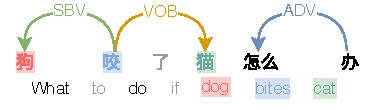
\includegraphics[scale=1.1]{figure/fig5-1-1.pdf}}

    \subfigure[被动语态(复述关系)]{\label{fig5-1-2}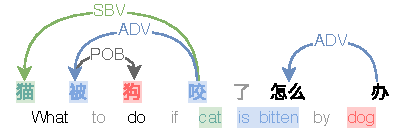
\includegraphics[scale=1.1]{figure/fig5-1-2.pdf}}

    \subfigure[被动语态(非复述关系)]{\label{fig5-1-3}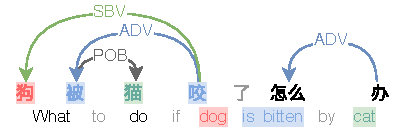
\includegraphics[scale=1.1]{figure/fig5-1-3.pdf}}
    \caption{主被动语态依存关系图}
    %Same words are with same color between example and corresponding translation.
    %'SBV'' to Subject-Predicate relation, 'ADV' refers to the relationship between adverbial and head word and 'POB' referfs to the relationship between preposition and object.
    \label{fig5-1}
\end{figure}

\subsection{语境特征}

语境(语言使用的场景)对语言表达有着一定的影响。
在大多数的非正式语境下,语言的表达有着随意性、简散性等特点,人类易懂但却对模型的鲁棒性提出了极大的挑战。
CQM$_{robust}$包含如下几种日常语境下的特征:

\begin{enumerate}
    \item \textbf{错别字:}
    在非正式书面用语中,错别字是最常见的一种语言错误。
    多数情况下,拼写错误并不影响人们的正常理解与交流,如例E30,{\kai“文身”}是网络上表达{\kai“纹身”}的一种常见错别字。
    神经网络模型也应该有能力察觉句子中的错别字并理解其真实意图,才能提高搜索引擎与问答系统等应用的容错率,提高用户体验感。
    \item \textbf{简单/复杂冗余:}
    冗余指的是句子中权重较低,对整句话的所传达的信息贡献不大仅用以凸显语境的部分,包括礼貌用语、问候、感叹等一些前置或后置的表达。
    如例E31与E32中的绿色部分,均为不同程度的冗余表达。
    该类别考察了模型的抗干扰能力,模型应当摒弃冗余表达的语义信息、捕获关键交互线索,
    借以判别出两个问句为语义相同的复述关系。
\end{enumerate}


\section{CQM$_{robust}$数据构造方案}

CQM$_{robust}$是一个多元化、自然化的中文数据集,其构建过程分为四个步骤。
如图~\ref{fig5-2}~所示,本章首先对源问题进行预处理操作,以便于加入符合语言学的扰动构造新问题。
然后,本章会对新问题进行是否为“自然语言”的检查,确保新问题必须是真实可靠的自然语言问句。
最后,本章将源问题和被扰乱的新问题配对作为一条样本,并由专门的数据审核人员对这些样本进行人工标注。
本小节将详细介绍CQM$_{robust}$的具体构建细节。

\begin{figure}[h]
    \centering
      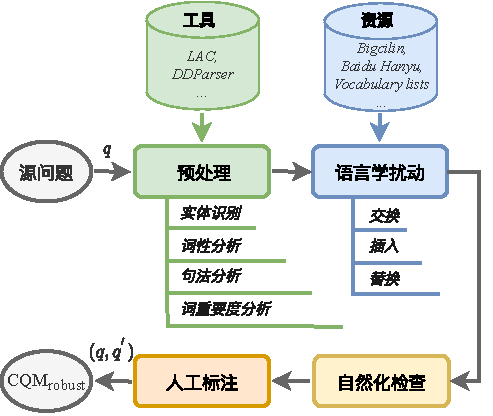
\includegraphics[scale=0.95]{figure/fig5-2.pdf}
    \caption{CQM$_{robust}$构造流程图}
    \label{fig5-2}
\end{figure}

\subsection{源问题预处理}

本节首先从百度搜索引擎的日志中收集了大量的源问题,所有的源问题都是用户提问的真实自然问句。
然后本章对源问题进行如下几个语言学预处理:

\begin{enumerate}
    \item \textbf{词性标注(Part-Of-Speech Tagging,简称POS Tagging):}
    借助百度中文词法分析工具(Lexical Analysis of Chinese,简称LAC)\footnote{https://github.com/baidu/lac}
    对源问题中的所有单词进行词性标注,便于体系化的对不同词性的词进行语言学扰动。
    \item \textbf{词重要性分析(Word Importance Analysis):}
    使用LAC工具标记出源问题中所有单词的权重(权重之和为1),单词的权重数值越大,则越能代表问句的语义走向。
    CQM$_{robust}$着重考察权重较高的词对源问题的影响。
    \item \textbf{命名实体识别(Named Entity Recognition,简称NER):}
    同样借助LAC工具标识出源问题中的实体,在小节~\ref{5.2.1 词法特征}~的命名实体子类别中详细介绍了如何利用这些实体设计测试样例。   
    \item \textbf{依存句法分析(Dependency Parsing):}
    借助百度依存句法分析工具(BaiDu Dependency Parser,简称DDParser)\footnote{https://github.com/baidu/DDParser}
    对源问句进行分析,
    从而设计相应的启发式规则构造如~\ref{5.2.2 句法特征}~小节所述的几种句法特征数据。
\end{enumerate}

\subsection{语言学扰动}

\begin{enumerate}
\item \textbf{词法特征:}
对于词法特征而言,
本章将源问题中的目标词替换为扰动词,或者将扰动词插入目标词前后。
所有的扰动词均通过如下几种方式收集:  
1) \textbf{Elasticsearch(简称ES)\footnote{https://github.com/elastic/elasticsearch}:}
从ES数据词典中检索与原词字面重叠的扰动词,如{\kai“空调”}和{\kai“空调扇”}。
2) \textbf{Faiss\footnote{https://github.com/facebookresearch/faiss}:}
从预先处理好的Faiss工具中查找与原词语义相近的扰动词,如{\kai“猕猴桃”}和{\kai“奇异果”}。
3) \textbf{Bigcilin\footnote{http://www.bigcilin.com/browser/}:}
从百度汉语词典中收集原词的同义词与反义词。
4) \textbf{XLM-RoBERTa\cite{conneau2019unsupervised}:}
将源问题中的目标词替换[MASK]特殊标记,
然后送入预训练语言模型XLM-RoBERTa中,
根据上下文预测出[MASK]位置的词作为扰动词。
5) \textbf{Vocabulary lists:}
本章预定义的一些特殊词汇表,如否定词表、时间词表。

\item \textbf{句法特征:}
对与句法特征而言,
本章首先从百度搜索日志中检索出与源问题编辑距离小于4的一些候选问题,
然后通过对比源问题与候选问题的依存结构,
将包含对称角色和非对称角色的问题对子保留,用于构造对应类别的测试样本。
同时,本章依据源问题和候选问题中的{\kai“被”}字特征以及主谓宾语法结构特征,
构造了一批主被动转换的样本。

\item \textbf{语境特征:}
本章借助中文错别字字典将源问题中的某一个字替换为常见的错别字。
对于冗余类别,本章插入一些疑问词、礼貌用语等在源问题中增加简单冗余表达,
并从百度高频问答日志中挑选一些长度差较大的复述问句作为复杂冗余样例。
\end{enumerate}


\subsection{自然化检查}

本章仅保留在近三个月的百度搜索日志中出现频率大于等于3次的扰动问句,以确保问句的质量和自然性,使得CQM$_{robust}$能有效地评估模型的实际应用能力。

\subsection{人工标注}

源问题和扰动问题组成的样例由百度内部数据团队进行人工审核。
首先,标注人员需要检查样本是否流畅、语法是否正确,以及标签(复述/非复述)是否合理。
低质量的样本将被丢弃,标签不合理样本的将被调整到其他测试类别或丢弃。
然后,这些样本将再由标注人员进行二轮审核,
每个样本由三位标注人员审核,两位或者两位以上的专家认同才算合格。
最终,从合格样本中随机选取10\%的样本由语言学专家进行审查,如果审查通过率小于95\%,
则数据团队需要对所有样本进行重新标注。

最终,CQM$_{robust}$包含10,121条高质量的自然问题对,表~\ref{table5-3}~和表~\ref{table5-2}~中分别展示了CQM$_{robust}$的统计信息与各个类别的详细信息。

% 表: train/dev/test description
\begin{table}
    \caption{CQM$_{robust}$数据统计}
    % \begin{spacing}{1.4}
    % \scriptsize
    \centering
    \newcommand{\tabincell}[2]{\begin{tabular}{@{}#1@{}}#2\end{tabular}}
    \setlength{\tabcolsep}{2mm}{
    \begin{tabular}{c|cc|ccc}
    \toprule[0.7pt]
    \multirow{2}{*}{\tabincell{c}{\textbf{类别}}} & \multicolumn{2}{c|}{\textbf{长度}} & \multicolumn{3}{c}{\textbf{数量}}  \\
      & \; 源问题\; & \;扰动问题 \; & \;复述 \; & \;非复述  & 全部  \\
    \midrule[0.7pt]
    \enspace{词法特征}\enspace  & 8.58 & 8.89  & 1,315 & 6,784  & 8,099               \\
    {句法特征}  & 9.86 & 9.89  & 678    & 532  & 1,210               \\
    {语境特征}   & 8.73    & 9.03    & 812  & 0 & 812                \\
    % {Speech Filler}     & 9.66    & 10.37   & 344  & 0   & 344                \\ 
    \midrule[0.7pt]
    \textbf{汇总}   & 8.74    & 8.90    & 2,805   & 7,316   & 1,0121              \\
    \bottomrule[0.7pt]
    \end{tabular}}
    \label{table5-3}
    % \end{spacing}
\end{table}

\section{实验及结果分析}

\subsection{数据集与评价方法}

本章在LCQMC数据集上对模型进行微调训练,并在CQM$_{robust}$上评估模型的性能。
LCQMC是由哈尔滨工业大学构造的一个大规模的中文问题复述语料库,数据集的详细介绍见~\ref{2.2 语料资源概述}~小节。

本章提倡除了采用传统的\textbf{微平均准确率(Micro-accuracy)}计算模型对CQM$_{robust}$中所有样本分类准确率的算术平均值,
还应当以样本类别为单位,采用\textbf{宏平均准确率(Macro-accuracy)}计算模型对32种不同数据分类准确率的算术平均值。
往往欺骗性越强的样本类别,其构造难度越大,即在CQM$_{robust}$中的样本数量越少。
采用宏平均准确率可以忽略多类别数据集中由样本数量差造成的性能偏差。


\subsection{基线模型与超参设置}

本章选用了6种采用不同预训练策略或参数规模的语言模型进行实验,包括:
$base$参数规模的BERT\cite{devlin2018bert}、ERNIE\cite{sun2019ernie}、RoBERTa\cite{liu2019roberta}和MacBERT\cite{cui2020revisiting}模型,
以及$large$参数规模的RoBERTa和MacBERT模型。
% BERT$_{base}$\cite{devlin2018bert}、ERNIE$_{base}$\cite{sun2019ernie}、
% RoBERTa$_{base}$RoBERTa$_{large}$\cite{liu2019roberta}
% MacBERT$_{base}$和MacBERT$_{large}$\cite{cui2020revisiting}。
本章所有模型输入问题对的最大长度限制为65,训练阶段batch\_size均设置为64。
对于${base}$规模的模型,优化器的学习率设置为5e-6,训练3轮。
对于${large}$规模的模型,优化器的学习率设置为2e-5,训练2轮。
为防止实验误差,本章的所有实验均进行3次取平均结果。


\subsection{CQM$_{robust}$评估结果分析}


\textbf{挑战性更高:}
表~\ref{table5-4}~展示了基线模型在LCQMC$_{test}$和CQM$_{robust}$上的评估结果。
其中,下标$b$表示模型为$base$规模,下标$l$表示模型为$large$规模,加粗和下划线分别标识出在测试集上表现最佳和第二的模型性能。
显而易见,所有模型在LCQMC$_{test}$上的准确率均高于87\%,
但是在CQM$_{robust}$上的性能却明显下降,$\triangle$表示两者性能差,最大性能差可达20.5\%。
由此说明,CQM$_{robust}$更具有挑战性,能有效地反应问题复述识别模型的真实能力。

% 表: 实验总体性能
\begin{table}
    \caption{LCQMC$_{test}$和CQM$_{robust}$实验性能对比}
    % \begin{spacing}{1.4}
    \centering
    % \scriptsize
    \newcommand{\tabincell}[2]{\begin{tabular}{@{}#1@{}}#2\end{tabular}}
    \begin{tabular}{c|c|c|c}
    \toprule[0.7pt]
    \textbf{模型} & \enspace \textbf{LCQMC$_{test}$}\enspace  & \enspace \textbf{CQM$_{robust}$} \enspace & \enspace \textbf{$\triangle$} \\
    \midrule[0.7pt]
    BERT\textsubscript{b} &87.1±0.1 &66.6±0.6 & \enspace -20.5\\
    ERNIE\textsubscript{b} & 87.3±0.1& 69.8±0.3 &\enspace -17.5 \\
    RoBERTa\textsubscript{b} & 87.2±0.4&69.5±0.1 &\enspace -17.7\\
    \enspace MacBERT\textsubscript{b}\enspace  &87.4±0.3 &70.3±0.6 &\enspace -17.1\\
    \hline
    RoBERTa\textsubscript{l} & \textbf{87.7±0.1}&\textbf{73.8±0.3} &\enspace -13.9\\
    MacBERT\textsubscript{l} &\underline{87.6±0.1} &\underline{73.8±0.5} &\enspace -13.8\\
    \bottomrule[0.7pt]
    \end{tabular}
    \label{table5-4}
    % \end{spacing}
\end{table}
    

\textbf{辨别能力更强:}
值得注意的是,所有的基线模型在LCQMC$_{test}$上均有着相近的性能结果,约为87\%。
但在CQM$_{robust}$上,$base$模型的性能从66.6\%到70.3\%不等,$large$模型的最高性能更是达到了73.8\%。
可以看出,CQM$_{robust}$能更加明显展现出模型的性能差异,对模型具有更高的区分度。

\textbf{评估角度更多样:}
CQM$_{robust}$是一个细粒度的评估基准,
其包含3大类特征类别、13个测试子类,共计32种数据测试项,
可以根据不同的语言现象对模型进行详细的评估。
本章采用多个基线模型在CQM$_{robust}$上的进行实验,实验结果如表~\ref{table5-2}~和表~\ref{table5-5}~所示。
通过对比不同模型在各个测试项上的表现差异,本节得出如下结论:

\begin{table}
    \caption{CQM$_{robust}$详细评估结果}
    % \begin{spacing}{1.1}
    % \scriptsize
    \centering
    \newcommand{\tabincell}[2]{\begin{tabular}{@{}#1@{}}#2\end{tabular}}
    \resizebox{155mm}{38mm}
    {
    \begin{tabular}{cc|cccccc|c|c|c|c}
    \toprule[0.7pt]
    \multicolumn{2}{c|}{\multirow{2}*{\textbf{\tabincell{c}{模型}}} }
     & \multicolumn{7}{c|}{\textbf{词法}} & \multirow{2}*{\textbf{句法}} & \multirow{2}*{\textbf{语境}} & \multirow{2}*{\textbf{CQM$_{robust}$}} \\
    \multicolumn{2}{c|}{ }& 基础词汇 & 命名实体 & 同义词 & 反义词 & 否定 & 时态 & \textbf{词法} &  &  & \\
     \midrule[0.7pt]
    \multirow{2}*{\tabincell{c}{BERT\textsubscript{b}}} & micro & 62.1±1.1 & 92.3±0.5 & 69.5±0.4 & 50.6±3.4 &
    64.4±5.9 & 35.1±3.3 & 67.2±0.7 & 59.1±0.4 &
    72.6±1.6 & 66.6±0.6  \\
    & macro & 51.9±1.5 & 91.2±0.7 & 76.4±0.6 & 50.6±3.4 &
    57.6±4.4 & 35.5±3.3 & 61.4±1.2 & 59.1±0.7 &
    71.1±1.1 & 62.0±0.9  \\\hline
    
    \multirow{2}*{\tabincell{c}{ERNIE\textsubscript{b}}} & micro & 64.6±0.5 & \underline{92.8±0.4} & 73.2±0.9 & 69.6±2.9 &
    77.8±1.1 & 48.0±1.9 & 71.0±0.3 & 60.0±1.2 &
    72.4±0.3 & 69.8±0.3  \\
    & macro & 52.4±0.7 & \underline{92.3±0.6} & 79.5±0.7 & 69.6±2.9 &
    69.1±1.2 & 48.5±1.9 & 65.5±0.5 & 56.5±1.0 &
    73.2±0.8 & 65.1±0.3  \\\hline
    
    \multirow{2}*{\tabincell{c}{RoBERTa\textsubscript{b}}} & micro & 64.2±0.1 & 90.6±1.8 & 74.2±1.4  &65.0±1.5 & 76.3±1.7 & 43.7±0.2 &
    70.1±0.1 & 63.1±0.6 & 73.3±0.1 & 69.5±0.1  \\
    & macro & 53.3±0.2 & 89.4±2.5 & 80.3±1.1 & 65.0±1.5 & 68.8±1.3 & 44.0±0.2 &
    65.0±0.1 & 60.9±0.6 & 75.6±0.5 & 65.5±0.1 \\\hline
    
    \multirow{2}*{\tabincell{c}{MacBERT\textsubscript{b}}} & micro & 64.8±1.1 & 92.0±0.7 & 73.3±1.1  & 73.1±4.3 & \underline{80.7±0.5} & 47.6±1.3 &
    71.2±0.7 & 62.1±1.0 & \underline{73.4±1.5} & 70.3±0.6  \\
    & macro & 54.2±0.9 & 90.7±0.6 & 79.7±0.5 & 73.1±4.6 & 70.7±0.1 & 47.7±0.2 &
    66.3±0.2 & 55.5±0.7 & 75.2±1.1 & 65.8±0.1  \\\hline
    
    \multirow{2}*{\tabincell{c}{RoBERTa\textsubscript{l}}} & micro & \textbf{67.2±0.9} &
    92.5±0.3 & \underline{76.0±2.1} & \textbf{91.7±2.3} & 80.2±0.8 & \textbf{58.6±2.8} &
    \underline{74.1±0.3} &
    \textbf{72.6±1.4} &
    73.2±1.9 &
    \textbf{73.8±0.3}  \\
    & macro & \textbf{57.7±0.6} &
    91.6±0.3 & \underline{81.7±1.6} & \textbf{91.7±2.3} & \underline{72.3±0.6} & \textbf{59.0±2.7} &
    \underline{70.2±0.3} &
    \textbf{63.4±1.2} &
    \underline{76.0±2.0} & \underline{69.8±0.2}  \\\hline
    
    \multirow{2}*{\tabincell{c}{MacBERT\textsubscript{l}}} & micro & \underline{65.6±0.8} &
    \textbf{93.2±0.6} & \textbf{83.2±1.6} & \underline{90.7±2.3} & \textbf{84.3±1.3} & \underline{55.5±4.0} &
    \textbf{74.4±0.4} &
    \underline{70.2±3.7} &
    \textbf{73.7±1.1} &
    \underline{73.8±0.5}  \\
    & macro & \underline{54.7±0.9} &
    \textbf{92.6±0.9} & \textbf{87.1±1.2} & \underline{90.7±2.3} & \textbf{78.1±0.9} & \underline{56.1±4.0} &
    \textbf{70.7±0.5} &
    \underline{61.6±2.4} &
    \textbf{77.1±0.6} & \textbf{70.2±0.5}  \\
    
    \bottomrule[0.7pt]
    \end{tabular}
    }
    \label{table5-5}
    % \end{spacing}
\end{table}
    
    % \setlength{\tabcolsep}{1.5mm}{

\begin{enumerate}
    \item 如表~\ref{table5-5}~所示,绝大部分测试类别的最优及次优性能集中在表格下半部分,即$large$模型的表现总体优于$base$模型。
    因为$large$模型的参数规模更大且训练语料更丰富,所以它们比$base$模型具有更强的能力。
    \item 在实体识别子类中,ERNIE$_{base}$的表现优于其他${base}$模型和RoBERTa$_{large}$模型,
    这是由于ERNIE在预训练的过程中加入了实体掩码策略,这有利于强化模型对实体词汇的识别能力。
    \item MacBERT$_{large}$模型在同义词子类表现最佳,这得益于它在预训练中采用了相近词掩码策略
    强化了模型对同义词的辨别能力。
    \item 所有模型在时态子类特征上的表现均较差,这说明模型对中文时间词所导致的语义差异缺乏敏感性。
    \item 在句法特征中,模型对于对称角色的感知能力要远远高于非对称角色。
    本文认为模型并未真正理解词语在句子中所扮演的角色,而仅仅是倾向于将字面重叠度高的两个问句判别为复述关系。
    \item ${base}$模型在错别字类别上表现要优于${large}$模型,
    这是由于${large}$模型的训练更加充分,间接导致了其对与错别字的感知更加敏感。
\end{enumerate}

\subsection{对抗训练分析}

CQM$_{robust}$是一个符合语言特征的自然问句数据集,有利于客观评估模型的鲁棒性。
为了证明这一点,本章使用两种对抗攻击产出的样本进行对抗训练实验,包括:
基于Wordnet的同义词替换攻击PWWS\cite{ren2019generating};基于Word2vec的同义词替换攻击TEXTFOOLER\cite{jin2020bert}。
并且,本章将这些强化后的模型在多种数据上进行交叉评估。
如表~\ref{table5-6}~所示,除了CQM$_{robust}$以外,
这些评估数据还包括:从对抗性样本中人工选取了200条自然样本子集PWWS\textsubscript{nat}和TEXTFOOLER\textsubscript{nat} ;
从CHECKLIST中文翻译数据中人工选取了400条问题对子集CHECKLIST\textsubscript{nat}。

% 表: 对抗数据量统计
\begin{table}
    % \begin{spacing}{1.4}
    \caption{对抗数据统计}
    \centering
    \footnotesize
    \newcommand{\tabincell}[2]{\begin{tabular}{@{}#1@{}}#2\end{tabular}}
    \setlength{\tabcolsep}{1.2mm}{
    \begin{tabular}{l|cc|cc|c}
    \toprule
    &PWWS & \enspace PWWS\textsubscript{nat} \enspace &\enspace TEXTFOOLER \enspace &\enspace TEXTFOOLER\textsubscript{nat} \enspace &\enspace CHECKLIST\textsubscript{nat}\\
    \midrule[0.7pt]
    训练数据\quad\ & \enspace 159,503\enspace&-& 64,086&-& \enspace -\\
    测试数据 &400&200&400&200&\enspace400 \\
    \bottomrule[0.7pt]
    \end{tabular}
    }
    \label{table5-6}
    % \end{spacing}
\end{table}
    

本章使用RoBERTa$_{large}$基线模型在LCQMC数据上进行对抗训练,实验结果如表~\ref{table5-7}~所示。
显而易见,经过对抗训练强化后的模型在PWWS和TEXTFOOLER测试数据上均有大幅提升。
但是,在经过人工筛选后的PWWS\textsubscript{nat}、TEXTFOOLER\textsubscript{nat}上,
并没有获得期望的性能提升。
同样,在CHECKLIST\textsubscript{nat}以及CQM$_{robust}$上也无明显提升,甚至略有下降。

% 表: 对抗训练性能结果
\begin{table*}[!h]
    \begin{spacing}{1.4}
    \scriptsize
    \caption{对抗训练性能对比} 
    \centering
    \newcommand{\tabincell}[2]{\begin{tabular}{@{}#1@{}}#2\end{tabular}}
    \begin{tabular}{lc|cc|cc|c|cc}
    \toprule[0.7pt]
    %  \multirow{2}*{\textbf{Model}} &
     \multirow{2}*{\textbf{训练数据}} & \multirow{2}*{\textbf{LCQMC}} & \multicolumn{4}{c|}{\textbf{对抗数据}} & \multirow{2}*{\textbf{CHECKLIST\textsubscript{nat}}} & \multicolumn{2}{c}{\textbf{CQM\textsubscript{robust}}} \\
     & & PWWS & PWWS\textsubscript{nat}& TEXTFOOLER & TEXTFOOLER\textsubscript{nat}& & Micro & Macro\\
    \midrule[0.7pt]
    
     LCQMC & \underline{87.7} & 58.1 & 81.5& 57.1 & 87.8& \underline{76.9} & \underline{73.8} & 69.8 \\
    
    %  LCQMC+PAWS &87.4\textcolor{textred}{\textsubscript{-0.3}} & 61.5\textcolor{textgreen}{\textsubscript{+3.4}} & 81.8\textcolor{textgreen}{\textsubscript{+0.3}}&58.3\textcolor{textgreen}{\textsubscript{+1.2}} & \underline{88.0}\textcolor{textgreen}{\textsubscript{+0.2}}& 76.4\textcolor{textred}{\textsubscript{-0.5}} & 73.2
    % \textcolor{textred}{\textsubscript{-0.6}} & \textbf{70.6}\textcolor{textgreen}{\textsubscript{+0.8}} \\
    
     LCQMC+PWWS & \underline{87.7}\textcolor{textgreen}{\textsubscript{+0.0}} & \textbf{97.6}\textcolor{textgreen}{\textsubscript{+39.5}} & 81.8\textcolor{textgreen}{\textsubscript{+0.3}}& \underline{73.1}\textcolor{textgreen}{\textsubscript{+16.0}} & 87.6\textcolor{textred}{\textsubscript{-0.2}}& 76.0\textcolor{textred}{\textsubscript{-0.9}} & \textbf{75.2}
    \textcolor{textgreen}{\textsubscript{+1.4}} & \underline{70.4}\textcolor{textgreen}{\textsubscript{+0.6}} \\
    
     LCQMC+FOOLER & 87.5\textcolor{textred}{\textsubscript{-0.2}} & \underline{78.5}\textcolor{textgreen}{\textsubscript{+20.4}} & \textbf{83.8}\textcolor{textgreen}{\textsubscript{+2.3}}& \textbf{80.8}\textcolor{textgreen}{\textsubscript{+23.7}} & 82.0\textcolor{textred}{\textsubscript{-5.8}}&\textbf{79.2}\textcolor{textgreen}{\textsubscript{+2.3}} & 71.4
    \textcolor{textred}{\textsubscript{-2.4}} & 68.8\textcolor{textred}{\textsubscript{-1.0}} \\
    
    % \midrule[0.4pt]
    
    % Ensemble & LCQMC &\textbf{88.0}\textcolor{textgreen}{$_{+0.3}$}&\underline{83.3}\textcolor{textgreen}{$_{+1.8}$} &60.3\textcolor{textgreen}{$_{+2.2}$}& \textbf{89.5}\textcolor{textgreen}{$_{+1.7}$}&54.3\textcolor{textred}{$_{-2.8}$}& 73.4\textcolor{textred}{$_{-3.5}$} & 72.0\textcolor{textred}{$_{-1.8}$} & 67.4\textcolor{textred}{$_{-2.4}$} \\
    
    
    \bottomrule[0.7pt]
    \end{tabular}
    \label{table5-7}
    \end{spacing}
\end{table*}

由此可见,常见的对抗性样本在自然评估数据集上效果并不明显,仅在与之分布一致的样本上有所效果。
作为一个符合语言学特征的自然化中文语料库,CQM$_{robust}$有利于模型的鲁棒性评估,
能够间接提高模型在现实世界中的应用能力。

\section{本章小结}

本章构造了一个多样化、自然化的中文数据集CQM$_{robust}$,用于评估问题识别复述模型的综合能力及鲁棒性。
CQM$_{robust}$包含3种语言特征、13个测试子类,共计32种蕴含不同语言学特征的测试项,其样本均来自于百度搜索日志中的用户真实提问。
实验证明,CQM$_{robust}$中的样本难度更大、更加具有挑战性,
且其细粒度的评估体系有助于诊断模型的优势与缺陷,使研究人员能够以更加多样化的方式分析模型。
